
\documentclass[aspectratio=169,11pt]{beamer}
\usepackage[T1]{fontenc}
\usepackage[utf8]{inputenc}
\usepackage[french]{babel}
\usepackage{lmodern}
\usepackage{graphicx}
\usepackage{tikz}
\usetikzlibrary{arrows.meta,positioning,calc,fit}

% --- Script du présentateur (décommenter pour l'afficher) ------------------
% \setbeameroption{show notes}
% \setbeameroption{show notes on second screen=right}   % nécessite pgfpages

% ---------------------------------------------------------------------------
%  Palette
% ---------------------------------------------------------------------------
\definecolor{colTitre}{RGB}{0,84,159}    % bleu profond
\definecolor{colOutil}{RGB}{35,120,75}   % vert (MCP)
\definecolor{colAccent}{RGB}{201,74,44}  % brique (risque)
\definecolor{colOr}{RGB}{190,140,0}      % or (connaissances)
\definecolor{colGris}{RGB}{90,98,110}
\definecolor{colFond}{RGB}{244,247,250}

% ---------------------------------------------------------------------------
%  Thème sobre
% ---------------------------------------------------------------------------
\usetheme{default}
\usefonttheme{professionalfonts}
\setbeamertemplate{navigation symbols}{}
\setbeamercolor{frametitle}{fg=colTitre,bg=white}
\setbeamerfont{frametitle}{series=\bfseries,size=\large}
\setbeamercolor{title}{fg=colTitre}
\setbeamercolor{structure}{fg=colTitre}
\setbeamercolor{block title}{fg=white,bg=colTitre}
\setbeamercolor{block body}{bg=colFond,fg=black}
\setbeamercolor{block title example}{fg=white,bg=colOutil}
\setbeamercolor{block body example}{bg=colOutil!8,fg=black}
\setbeamertemplate{blocks}[rounded][shadow=false]
\setbeamertemplate{itemize items}[circle]
\setbeamercolor{itemize item}{fg=colAccent}
\setbeamercolor{itemize subitem}{fg=colOutil}

\setbeamertemplate{frametitle}{%
  \vspace{0.35em}\hspace{0.2em}\insertframetitle\par
  \vspace{-0.35em}{\color{colTitre!30}\rule{\textwidth}{0.6pt}}}

\setbeamertemplate{footline}{%
  \leavevmode\hbox{%
    \begin{beamercolorbox}[wd=\paperwidth,ht=2.6ex,dp=1.1ex,rightskip=1.1em]{}%
      \hfill\scriptsize\color{colGris}\insertframenumber%
    \end{beamercolorbox}}%
}

% ===========================================================================
\begin{document}

% ---------------------------------------------------------------------------
% DIAPO 1 — PAGE DE GARDE
% ---------------------------------------------------------------------------
\begin{frame}[plain]
  \vfill
  \begin{center}
    {\color{colTitre}\rule{0.55\textwidth}{1.3pt}}\\[0.9em]
    {\LARGE\bfseries\color{colTitre}Int\'egration du framework MITRE ATT\&CK\\[0.2em]
      dans un \'ecosyst\`eme MCP pour la d\'etection\par}
    \vspace{0.6em}
    
    \vspace{1.3em}
    {\large\bfseries Kamil Saleh\par}
    \vspace{0.5em}
    {\small\color{colGris}Superviseurs UQAC : Kevin Bouchard \textbullet{}
      Fehmi Jaafar\par}
    {\small\color{colGris}Superviseur Hydro-Qu\'ebec : Franck Jeannot\par}
    \vspace{0.7em}
  
  \end{center}
  \vfill
  
\end{frame}

% ---------------------------------------------------------------------------
% DIAPO 2 — MISE EN CONTEXTE : problèmes, premières tentatives, RAG, MCP
% ---------------------------------------------------------------------------
\begin{frame}
  \frametitle{Le contexte : une IA brillante\ldots{} qui ne dit jamais
    \og je ne sais pas \fg}
  \vspace{0.55cm}
  \begin{center}
  \scalebox{0.96}{%
  \begin{tikzpicture}[
    etape/.style={rectangle, rounded corners=3pt, draw, thick, align=center,
      text width=2.9cm, minimum height=2.0cm, font=\footnotesize,
      inner sep=4pt},
    fleche/.style={-{Stealth[length=3mm]}, thick, colGris}]
    \node[etape, draw=colTitre, fill=colTitre!8, right=0.45cm of p] (t)
      {\textbf{Les premi\`eres tentatives}\\[4pt]
       \scriptsize TRAM plafonne (annotation) ;\\
       LLM seuls : $F_1$ $0{,}64$ au mieux.};
    \node[etape, draw=colOr!80!black, fill=colFond, right=0.45cm of t] (r)
      {\textbf{L'ancrage par RAG}\\[4pt]
       \scriptsize Jusqu'\`a $F_1 \approx 0{,}90$\ldots{}\\
       mais l'implicite \'echappe.};
    \node[etape, draw=colOutil, very thick, fill=colOutil!8,
      right=0.45cm of r] (m)
      {\textbf{L'ancrage par outils}\\[4pt]
       \scriptsize Le mod\`ele \textbf{consulte}\\ la source
       officielle.\\[3pt]
       {\color{colOutil}\bfseries le MCP notre approche}};
    \draw[fleche] (p) -- (t);
    \draw[fleche] (t) -- (r);
    \draw[fleche] (r) -- (m);
  \end{tikzpicture}}
  \end{center}
  \vspace{0.55cm}
  \begin{center}
    \small\color{colTitre}\bfseries Capables, mais pas dignes de confiance
    seuls, la fiabilité tient \`a l'ancrage.
  \end{center}
\end{frame}

% ---------------------------------------------------------------------------
% DIAPO 3 — C'EST QUOI LE MCP : définition + analogie USB + comparaison
% ---------------------------------------------------------------------------
\begin{frame}
  \frametitle{C'est quoi, le MCP ?}
  \vspace{0.05cm}
  \begin{block}{}
    \small Le \textbf{Model Context Protocol} (MCP) : un standard
    ouvert (2024) qui branche un mod\`ele d'IA sur une source de donn\'ees
    par des appels trac\'es.
  \end{block}
  \vspace{0.15cm}
  \begin{center}
  \begin{tikzpicture}[font=\scriptsize,
    a/.style={rectangle, rounded corners=3pt, draw, thick, align=center,
      minimum height=0.85cm, text width=2.35cm, inner sep=3pt},
    fl/.style={{Stealth[length=2.2mm]}-{Stealth[length=2.2mm]}, thick,
      colGris}]
    \node[a, draw=colTitre, fill=colTitre!8] (llm)
      {\textbf{LLM}\\ \scriptsize l'ordinateur};
    \node[a, draw=colGris, fill=colGris!8, right=0.9cm of llm] (cli)
      {\textbf{Client MCP}\\ \scriptsize le hub USB-C};
    \node[a, draw=colOutil, fill=colOutil!8, right=0.9cm of cli] (srv)
      {\textbf{Serveur MCP}\\ \scriptsize la cl\'e USB};
    \draw[fl] (llm)--(cli);
    \draw[fl] (cli)--(srv);
  \end{tikzpicture}
  \end{center}
  \vspace{0.15cm}
  \begin{columns}[T]
    \begin{column}{0.32\textwidth}
     
    \end{column}
  \end{columns}
  \vspace{0.25cm}

  \note{\scriptsize
    C'est quoi, le MCP ? Le Model Context Protocol : un standard ouvert qui
    branche un mod\`ele d'IA sur une source de donn\'ees par des appels
    trac\'es.\\[2pt]
    L'image la plus simple : le LLM, c'est l'ordinateur ; le client MCP,
    c'est son hub USB-C ; et un serveur MCP, c'est une cl\'e USB. On branche
    la cl\'e, l'ordinateur sait la lire --- quelle que soit la marque. Notre
    serveur MITRE est une de ces cl\'es.\\[2pt]
    La diff\'erence avec les autres approches : un LLM seul r\'ecite de
    m\'emoire --- et se trompe sans qu'on le voie. Le RAG colle des extraits
    ressemblants dans le contexte --- mieux, mais passif. Avec le MCP, le
    mod\`ele consulte la source officielle : chaque r\'eponse est sourc\'ee,
    dat\'ee, trac\'ee. Et comme c'est un standard : \'ecrit une fois,
    branch\'e partout.}
\end{frame}

% ---------------------------------------------------------------------------
% DIAPO 4 — NOTRE SOLUTION : le serveur MCP (le trajet d'une requête)
% ---------------------------------------------------------------------------
\begin{frame}
  \frametitle{Notre serveur MCP : le trajet d'une requ\^ete}
  \vspace{0.2cm}
  \begin{center}
  \scalebox{0.94}{%
  \begin{tikzpicture}[font=\scriptsize,
    blk/.style={rectangle, rounded corners=2.5pt, draw, thick, align=center,
      minimum height=0.85cm, text width=1.85cm, inner sep=3pt},
    io/.style={rectangle, rounded corners=2.5pt, draw=colGris!70,
      fill=colGris!8, align=center, minimum height=0.72cm, text width=1.35cm,
      inner sep=3pt},
    dbb/.style={rectangle, rounded corners=2.5pt, draw=colOr!80!black,
      fill=colFond, align=center, text width=2.1cm, inner sep=3pt,
      minimum height=0.8cm},
    fl/.style={-{Stealth[length=2.4mm]}, thick, colGris}]
    \node[io] (in) {JSON-RPC\\ \scriptsize requ\^ete};
    \node[blk, draw=colTitre, fill=colTitre!8, right=0.42cm of in] (rout)
      {\textbf{D\'ecodage}\\ routage};
    \node[blk, draw=colTitre, fill=colTitre!8, right=0.42cm of rout] (val)
      {\textbf{Validation}\\ types, longueurs};
    \node[blk, draw=colOutil, fill=colOutil!8, right=0.42cm of val] (mot)
      {\textbf{Moteur}\\ mapping, scoring};
    \node[blk, draw=colAccent, fill=colAccent!8, right=0.42cm of mot] (ser)
      {\textbf{S\'erialisation}\\ + \texttt{db\_version}};
    \node[io, right=0.42cm of ser] (out) {JSON-RPC\\ \scriptsize r\'eponse};
    \draw[fl] (in)--(rout); \draw[fl] (rout)--(val); \draw[fl] (val)--(mot);
    \draw[fl] (mot)--(ser); \draw[fl] (ser)--(out);
    \node[dbb, below=0.8cm of mot] (base)
      {Base ATT\&CK E+ICS\\ versionn\'ee};
    \node[dbb, left=0.7cm of base, text width=1.9cm] (thq)
      {R\'ef\'erentiel\\ interne};
    \node[dbb, below=0.8cm of ser, text width=1.9cm, draw=colGris!70] (aud)
      {Journal d'audit};
    \draw[{Stealth[length=2.4mm]}-{Stealth[length=2.4mm]}, colGris!70]
      (mot)--(base);
    \draw[{Stealth[length=2.4mm]}-{Stealth[length=2.4mm]}, colOr!80!black,
      thick] (thq)-- node[below,font=\scriptsize,colOr!70!black,
      yshift=0.3mm]{\'etend} (base);
    \draw[fl, colGris!70] (ser)--(aud);
  \end{tikzpicture}}
  \end{center}
  \vspace{0.2cm}
  \begin{tikzpicture}
    \node[rectangle, rounded corners=3pt, draw=colOutil, very thick,
      fill=colOutil!6, inner sep=6pt, text width=0.955\textwidth] {%
      {\small\bfseries\color{colOutil}Le moteur : proposer, puis
       v\'erifier}\\[2pt]
      \footnotesize
      \texttt{search\_techniques} : \textbf{candidats scor\'es + preuves}
      \;$\rightarrow$\; \texttt{get\_technique} : \textbf{d\'efinition
      compl\`ete} \;$\rightarrow$\; \og\textbf{pas de mapping}\fg{}
      est valide.};
  \end{tikzpicture}
  \note{\scriptsize
    Voici notre solution : le serveur MCP lui-m\^eme. Un seul fichier Python,
    biblioth\`eque standard uniquement --- auditable ligne par ligne --- et en
    lecture seule par conception. Suivons une requ\^ete. Elle arrive en
    JSON-RPC ; le serveur la d\'ecode et la route --- et m\^eme un appel \`a
    un outil qui n'existe pas laisse une trace, car c'est la signature d'une
    hallucination d'outil. Ensuite, validation avant tout traitement : types,
    longueurs, caract\`eres de contr\^ole --- une entr\'ee malform\'ee est
    rejet\'ee, et le refus est trac\'e. Puis le moteur travaille : recherche
    par mots entiers avec racinisation, sur des index pr\'ecalcul\'es ; un
    score normalis\'e entre 0 et 1 qui mesure la couverture de la question ;
    et des preuves --- les mots r\'eellement trouv\'es. Il s'appuie sur la
    base ATT\&CK Enterprise + ICS, versionn\'ee, o\`u une technique
    r\'evoqu\'ee est redirig\'ee au lieu de dispara\^itre --- et sur notre
    r\'ef\'erentiel interne, qui l'\'etend, accroch\'e aux techniques MITRE.
    La r\'eponse est s\'erialis\'ee avec la version de la base
    (\texttt{db\_version}) et repart en JSON-RPC. Et transversalement, chaque
    \'ev\'enement --- appel, refus, erreur --- laisse une ligne dans le
    journal d'audit.\\[2pt]
    Le moteur encode une m\'ethode en deux temps : \emph{proposer} --- des
    candidats scor\'es avec preuves --- puis \emph{v\'erifier} --- par la
    d\'efinition compl\`ete. Et \og pas de mapping \fg{} est une conclusion
    valide : le serveur l'\'ecrit lui-m\^eme.}
\end{frame}

% ---------------------------------------------------------------------------
% DIAPO 5 — CE QUE ÇA RAPPORTE À HYDRO-QUÉBEC (avantages)
% ---------------------------------------------------------------------------
\begin{frame}
  \frametitle{Ce que \c{c}a rapporte \`a Hydro-Qu\'ebec}
  \vspace{0.15cm}
  \begin{columns}[T]
    \begin{column}{0.485\textwidth}
      \begin{block}{Versionnage \& mise \`a jour}
        \footnotesize \textbf{La version ATT\&CK de notre choix}, chaque
        r\'eponse dat\'ee ; le r\'ef\'erentiel vivant suivi \`a la source,
        \textbf{sans r\'eentra\^iner} de mod\`ele.
      \end{block}
      \vspace{0.25cm}
      \begin{block}{Hallucination ma\^itris\'ee}
        \footnotesize Un identifiant retourn\'e \textbf{existe forc\'ement}
        dans la base. Ex. : \texttt{T1086} r\'evoqu\'ee $\rightarrow$
        redirig\'ee vers \texttt{T1059.001}.
      \end{block}
    \end{column}
    \begin{column}{0.485\textwidth}
      \begin{block}{Customisation interne}
        \footnotesize Nos rapports red team et CTI avec des ID MITRE en Interne.
      \end{block}
      \vspace{0.25cm}
      \begin{exampleblock}{Polyvalence}
        \footnotesize \ldots{}
        Trois cas d'utilisation $\rightarrow$ les diapos suivantes.
      \end{exampleblock}
    \end{column}
  \end{columns}
\end{frame}

% ---------------------------------------------------------------------------
% DIAPO 6 — CAS D'UTILISATION 1 : l'interface de chat n8n
% ---------------------------------------------------------------------------
\begin{frame}
  \frametitle{Cas d'utilisation 1 : l'interface de chat n8n}
  \vspace{0.1cm}
  \begin{center}
    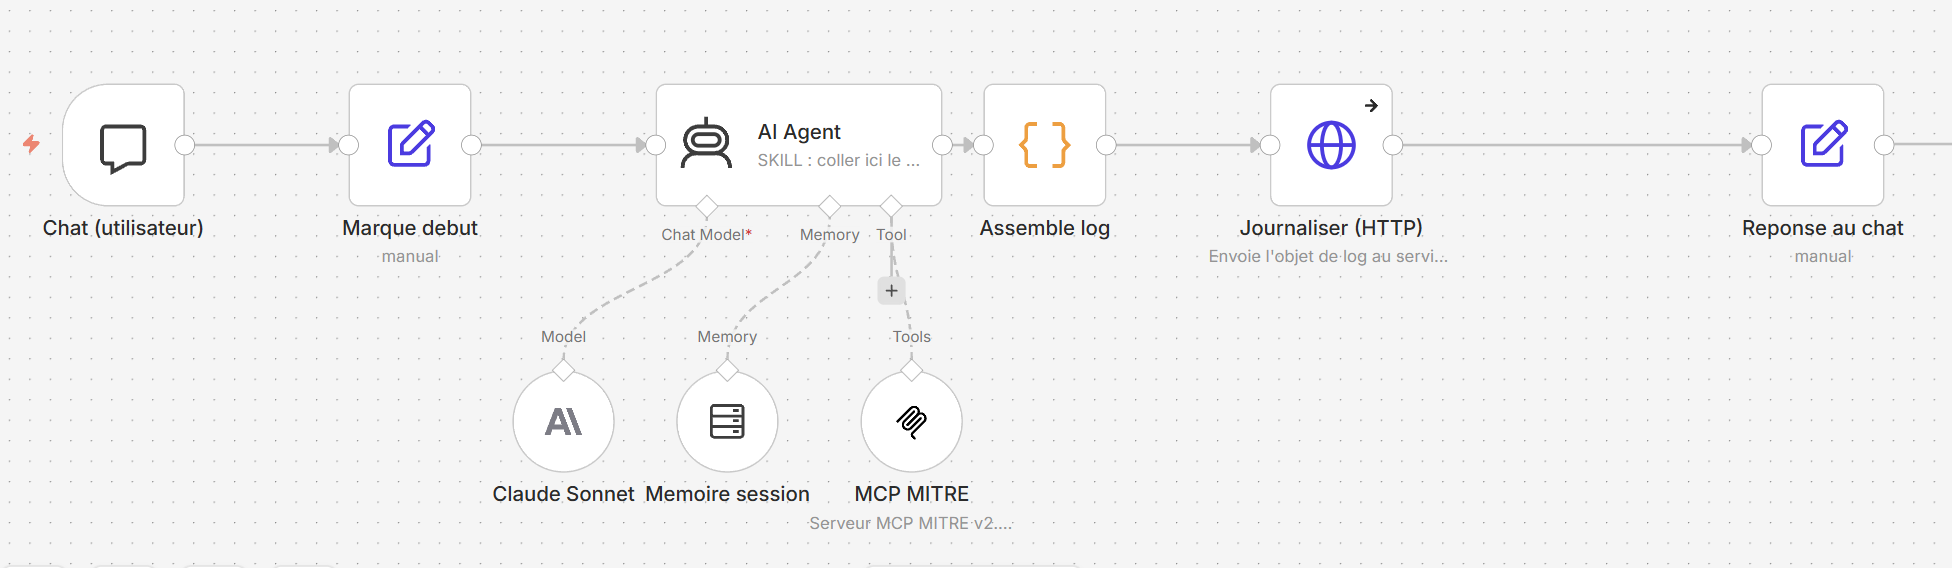
\includegraphics[width=0.98\textwidth]{workflow_n8n.png}
  \end{center}
  \vspace{0.15cm}
  {\footnotesize
   \makebox[0.45cm][l]{\textcolor{colAccent}{\textbf{1}}}Question de
   l'analyste \;$\rightarrow$\;
   \makebox[0.45cm][l]{\textcolor{colAccent}{\textbf{2}}}l'agent appelle le
   \textbf{serveur MCP MITRE} \;$\rightarrow$\;
   \makebox[0.45cm][l]{\textcolor{colAccent}{\textbf{3}}}chaque appel
   \textbf{journalis\'e} \;$\rightarrow$\;
   \makebox[0.45cm][l]{\textcolor{colAccent}{\textbf{4}}}r\'eponse
   \textbf{sourc\'ee et dat\'ee}.\par}
  \note{\scriptsize
    Premier cas d'utilisation, tel qu'il tourne aujourd'hui : une interface
    de chat dans n8n. \`A gauche, l'analyste pose sa question en langage
    naturel --- un journal, une alerte. L'agent d'IA, motoris\'e par Claude
    avec une m\'emoire de session, raisonne et appelle notre serveur MCP
    MITRE. Chaque appel est assembl\'e et journalis\'e par HTTP --- notre
    piste d'audit, l'auditabilit\'e qu'exige la loi canadienne sur la
    protection des cybersyst\`emes essentiels. Et l'analyste re\c{c}oit une
    r\'eponse sourc\'ee et dat\'ee --- rien de m\'emoire.\\[2pt]
    Voil\`a pour le prototype qui tourne. Maintenant : qu'est-ce que
    \c{c}a apporte \`a Hydro-Qu\'ebec ?}
\end{frame}

% ---------------------------------------------------------------------------
% DIAPO 7 — CAS D'UTILISATION 2 : les rapports CTI
% ---------------------------------------------------------------------------
\begin{frame}
  \frametitle{Cas d'utilisation 2 : les rapports CTI}
  \vspace{0.35cm}
  \begin{center}
  \scalebox{0.90}{%
  \begin{tikzpicture}[font=\scriptsize,
    b/.style={rectangle, rounded corners=3pt, draw, thick, align=center,
      minimum height=0.95cm, inner sep=4pt, text width=2.15cm},
    fl/.style={-{Stealth[length=2.6mm]}, thick, colGris}]
    \node[b, draw=colGris, fill=colGris!8] (cti)
      {\textbf{Rapport CTI}\\ \scriptsize public ou interne};
    \node[b, draw=colTitre, fill=colTitre!8, right=0.75cm of cti] (ext)
      {\textbf{Extraction}\\ \scriptsize comportements\\ observables};
    \node[b, draw=colOutil, fill=colOutil!8, right=0.75cm of ext] (prop)
      {\textbf{Proposition}\\ \scriptsize candidats scor\'es\\ + preuves};
    \node[b, draw=colOutil, fill=colOutil!8, right=0.75cm of prop] (ver)
      {\textbf{V\'erification}\\ \scriptsize d\'efinition\\ compl\`ete};
    \node[b, draw=colAccent, fill=colAccent!8, right=0.75cm of ver] (val)
      {\textbf{Validation}\\ \scriptsize humaine};
    \draw[fl] (cti)--(ext); \draw[fl] (ext)--(prop);
    \draw[fl] (prop)--(ver); \draw[fl] (ver)--(val);
    \node[below=0.55cm of prop, rectangle, rounded corners=3pt,
      draw=colOr!80!black, fill=colFond, inner sep=4pt, text width=2.3cm,
      align=center] (base) {Base ATT\&CK\\ E+ICS versionn\'ee};
    \draw[{Stealth[length=2.4mm]}-{Stealth[length=2.4mm]}, colOr!80!black]
      (prop)--(base);
    \draw[{Stealth[length=2.4mm]}-{Stealth[length=2.4mm]}, colOr!80!black]
      (ver.south)--(base.north east);
    \node[below=0.55cm of ver, xshift=1.7cm, rectangle, rounded corners=3pt,
      draw=colGris!70, fill=colGris!6, inner sep=4pt, text width=2.1cm,
      align=center] (aud) {Journal d'audit};
    \draw[fl, colGris!70] (ver.south east)--(aud.north);
  \end{tikzpicture}}
  \end{center}
  \vspace{0.4cm}
  \begin{center}\small
    Des heures de lecture experte $\rightarrow$ quelques minutes de
    validation \og pas de mapping \fg{} reste valide.
  \end{center}
 
\end{frame}

% ---------------------------------------------------------------------------
% DIAPO 8 — CAS D'UTILISATION 3 : un agent, plusieurs serveurs MCP
% ---------------------------------------------------------------------------
\begin{frame}
  \frametitle{Cas d'utilisation 3 : un agent, plusieurs serveurs MCP}
  \vspace{0.15cm}
  \begin{center}
  \begin{tikzpicture}[font=\scriptsize,
    b/.style={rectangle, rounded corners=3pt, draw, thick, align=center,
      minimum height=0.8cm, inner sep=4pt},
    chip/.style={rectangle, rounded corners=3pt, draw, thick, align=center,
      minimum height=0.68cm, text width=2.9cm, inner sep=3pt},
    fl/.style={{Stealth[length=2.4mm]}-{Stealth[length=2.4mm]}, thick}]
    \node[b, draw=colTitre, fill=colTitre!8, text width=2.3cm,
      minimum height=1.5cm] (agent) at (0,0)
      {\textbf{Agent (LLM)}\\ \scriptsize orchestre les appels};
    \node[b, draw=colGris, fill=colGris!8, text width=1.5cm,
      left=0.8cm of agent] (an) {Analyste};
    \node[chip, draw=colOutil, fill=colOutil!8]  (m1) at (5.4, 2.0)
      {MCP \textbf{ATT\&CK}};
    \node[chip, draw=colOutil, fill=colOutil!8]  (m2) at (5.4, 1.2)
      {MCP \textbf{ATLAS}};
    \node[chip, draw=colTitre!70, fill=colTitre!6] (m3) at (5.4, 0.4)
      {MCP \textbf{SIEM}};
    \node[chip, draw=colTitre!70, fill=colTitre!6] (m4) at (5.4,-0.4)
      {MCP \textbf{IDS}};
    \node[chip, draw=colOr!80!black, fill=colOr!10] (m5) at (5.4,-1.2)
      {MCP \textbf{rapports CTI}\\[-1pt] {\tiny red team}};
    \node[chip, draw=colOr!80!black, fill=colOr!10] (m6) at (5.4,-2.0)
      {MCP \textbf{Confluence}};
    \node[font=\small, colGris] at (5.4,-2.6) {\ldots};
    \draw[fl, colGris] (an)--(agent);
    \draw[fl, colOutil]      (agent.east) -- (m1.west);
    \draw[fl, colOutil]      (agent.east) --
      node[above, font=\scriptsize\bfseries, colOutil, pos=0.45]{MCP}
      (m2.west);
    \draw[fl, colTitre!70]   (agent.east) -- (m3.west);
    \draw[fl, colTitre!70]   (agent.east) -- (m4.west);
    \draw[fl, colOr!80!black] (agent.east) -- (m5.west);
    \draw[fl, colOr!80!black] (agent.east) -- (m6.west);
    \node[b, draw=colGris!70, fill=colGris!6, text width=2.0cm,
      minimum height=0.55cm] (aud) at (0,-2.3)
      {\scriptsize Journal d'audit};
    \draw[-{Stealth[length=2.4mm]}, thick, colGris!70] (agent)--(aud);
  \end{tikzpicture}
  \end{center}
  \vspace{0.15cm}
  \begin{center}\small
  \end{center}

\end{frame}

% ---------------------------------------------------------------------------
% DIAPO 9 — LE MCP, UNE SURFACE D'ATTAQUE + mesures de sécurité
% ---------------------------------------------------------------------------
\begin{frame}
  \frametitle{Le MCP : un outil mais aussi une surface d'attaque}
  \vspace{0.1cm}
  \begin{block}{}
    \small Un LLM isol\'e qui se trompe produit du texte, branch\'e
    \`a des outils, il peut produire une \textbf{action}.
  \end{block}
  \vspace{0.2cm}
  \begin{center}
  {\footnotesize
  \renewcommand{\arraystretch}{1.15}
  \begin{tabular}{@{}p{0.42\textwidth}p{0.52\textwidth}@{}}
    {\color{colAccent}\bfseries Menace document\'ee} &
    {\color{colTitre}\bfseries Mesure \`a pr\'evoir dans notre serveur} \\[1pt]
    \hline
    Empoisonnement d'outil\newline
      {\scriptsize\itshape\color{colGris}tool poisoning} &
      Descriptions fig\'ees et versionn\'ees, int\'egrit\'e v\'erifi\'ee \\
    Injection indirecte de prompt\newline
      {\scriptsize\itshape\color{colGris}indirect prompt injection} &
      S\'eparation donn\'ees / instructions, validation des entr\'ees \\
    Acc\`es non autoris\'e\newline
      {\scriptsize\itshape\color{colGris}unauthorized access} &
      Authentification par jeton + chiffrement (TLS) \\
    Action ou exfiltration non voulue\newline
      {\scriptsize\itshape\color{colGris}unintended action / exfiltration} &
      Lecture seule, moindre privil\`ege \\
    D\'eni de service\newline
      {\scriptsize\itshape\color{colGris}denial of service} &
      Limitation de d\'ebit \\
    Perte de tra\c{c}abilit\'e\newline
      {\scriptsize\itshape\color{colGris}loss of auditability} &
      Journal d'audit : chaque appel \emph{et} chaque refus \\
  \end{tabular}}
  \end{center}
  \note{\scriptsize
    Je termine sur une lucidit\'e n\'ecessaire : le MCP est un outil, mais
    c'est aussi une surface d'attaque. La litt\'erature l'a mesur\'e sur des
    serveurs r\'eels : le banc d'essai MCPTox, publi\'e \`a AAAI 2026, montre
    que l'empoisonnement d'outil --- glisser des instructions malveillantes
    dans la description m\^eme d'un outil --- r\'eussit en moyenne dans 36,5\,\%
    des cas, et que les mod\`eles les plus capables sont souvent les plus
    vuln\'erables. Et des vuln\'erabilit\'es critiques ont d\'ej\`a \'et\'e
    publi\'ees, comme la CVE-2025-6514, cot\'ee 9,6 sur 10, qui permettait
    l'ex\'ecution de commandes arbitraires via un utilitaire MCP.\\[2pt]
    C'est pourquoi la s\'ecurit\'e n'est pas un ajout mais une partie du
    projet : \`a chaque menace document\'ee correspond une mesure \`a
    pr\'evoir dans notre serveur ---
    descriptions d'outils fig\'ees et versionn\'ees, validation des entr\'ees,
    authentification, lecture seule par conception, limitation de d\'ebit, et
    un journal d'audit qui trace chaque appel et chaque refus. Un outil d'aide
    \`a la d\'etection qui deviendrait lui-m\^eme un vecteur d'attaque serait
    une r\'egression.}
\end{frame}

% ---------------------------------------------------------------------------
% DIAPO 10 — QUESTIONS
% ---------------------------------------------------------------------------
\begin{frame}
  \vfill
  \begin{center}
    {\color{colTitre}\rule{0.3\textwidth}{1.2pt}}\\[1.2em]
    {\Large\bfseries\color{colTitre}Questions ?\par}
    \vspace{1.0em}
    {\color{colTitre}\rule{0.3\textwidth}{1.2pt}}
  \end{center}
  \vfill
  \note{\scriptsize
    Merci de votre attention. Je r\'esume en une phrase : un LLM ancr\'e sur
    MITRE ATT\&CK par un serveur MCP interne, c'est un assistant qui cite ses
    sources, qui reste \`a jour, qui conna\^it \emph{notre} contexte --- et
    dont chaque r\'eponse est auditable. Je prends vos questions avec
    plaisir.}
\end{frame}

\end{document}
